\documentclass[10pt,a4paper,twoside]{report}

\input{../../base/BasePackage.sty}
\input{../../base/OptionsListingC++.sty}

\usepackage{newalg}

% Mettre des hyperliens dans le pdf
\hypersetup{pdftitle={Projet méthode d'optimisation},
  pdfsubject={Projet d'informatique - Magistère de Physique Fondamentale},
  pdfauthor={Xavier Garrido, LAL,
    <garrido@lal.in2p3.fr>},
  pdfkeywords={optimisation, simulated annealing, C++}
}

\begin{document}
\renewcommand{\chaptername}{Projet}

\setcounter{chapter}{0}
\chapter{Méthode d'optimisation : \emph{Simulated Annealing} ou "le recuit simulé"}
\label{projet::simulated_annealing}

\section{Historique}

La méthode de "recuit simulé" ou \emph{simulated
  annealing}~\cite{kirk1,kirk2} est un algorithme d'optimisation. En
mathématiques, l'optimisation consiste en la recherche de minimum
d'une fonction donnée: le domaine d'application couvre ainsi des
disciplines aussi diverses que l'informatique et la génétique en
passant, entre autres, par la physique\footnote{de telles approches
  souffrent toutefois d'une certaine forme de discrédit au sein de la
  communauté physicienne. La principale raison tient à leur important
  "contenu" mathématique qui a tendance à rebuter le physicien
  \emph{lambda}. Nous verrons néanmoins que cette réputation est
  largement surfaite et que la mise en \oe uvre de telles méthodes ne
  présentent pas de réelles difficultés.}.

Historiquement, la méthode de "recuit simulé" tire son nom et son
inspiration de pratiques issues de la thermodynamique et plus
particulièrement, de la façon dont les métaux sont chauffés puis
refroidis. En métallurgie, le recuit d'une pièce métallique est un
procédé correspondant à un cycle de chauffage, maintien en température
puis refroidissement controlé permettant de modifier les
caractéristiques de ce métal. \`A l'origine, les atomes qui composent
le métal sont pris dans une structure cristalline solide. Lorsque le
métal est chauffé, l'énergie disponible permet aux molécules de briser
leurs liaisons chimiques rendant aux atomes, leur mobilité. Si le
métal est refroidi lentement, la mobilité thermique diminue et les
atomes cherchent à former de nouvelles liaisons. Chose surprenante,
ils se répartissent souvent de manière plus régulière vis-à-vis de
leur configuration initiale. Du point de vue chimique, la stabilité du
métal tient à l'agencement des atomes et au fait que leurs états
respectifs atteint alors un minimum global d'énergie. Si tout est fait
dans les règles de l'art, le métal devient plus souple, plus flexible
et présente moins d'irrégularités\footnote{ce procédé est notamment
  utilisé lors de la fabrication de semi-conducteurs en silicium pour
  les microprocesseurs et les modules de mémoire des ordinateurs. Ces
  composants nécessitent un cristal de silicium extrêmement pur, ne
  présentant en particulier aucune irrégularité.}. Dans le cas
contraire, si le métal est refroidi brusquement, il atteint un état
"instable", polycristallin d'énergie plus élevée.

Le c\oe ur du processus est ainsi un refroidissement lent, autorisant
des temps suffisamment longs pour que les atomes se redistribuent au
fur et à mesure que leur mobilité diminue. Physiquement, le mécanisme
naturel de minimisation de l'énergie repose sur la distribution de
probabilité de Boltzmann
\begin{equation}
  p(E)\propto\exp\left(-E/kT\right)
  \label{eq:Boltz}
\end{equation}
Cette équation traduit le fait qu'un système à l'équilibre thermique à
la température $T$, présente une distribution de ces états
d'énergie~$E$. \`A basse température, il est possible, bien que la
probabilité soit infime, de trouver le système dans un état de grande
énergie. Cependant, il existe également une probabilité complémentaire
autorisant le système à rejoindre un état de moindre énergie;
l'objectif final étant de parvenir d'un état métastable correspondant
à un minimium local d'énergie, à l'état stable de plus basse
énergie. Ce faisant, le système "emprunte" ponctuellement des états
de plus haute énergie, d'autant plus défavorisés que la température
est faible, mais qui, à terme, lui permettront de rejoindre l'état
d'énergie minimum.

La probabilité qu'un système thermodynamique passe d'un état d'énergie
$E_1$ à un état d'énergie $E_2$, est donc égale à
$p=\exp\left[-(E_2-E_1)/kT\right]$. Si $E_1>E_2$, la probabilité $p$
est toujours plus grande que~1, le système choisira systématiquement
cette nouvelle configuration. Toutefois, un état de plus grande
énergie sera toléré avec une probabilité $p$ d'autant plus faible que
la température sera minime.

Metropolis~\emph{et al.}~\cite{metro} furent les premiers à
implémenter, dès 1953, ce type de principe dans le calcul
numérique. Inévitablement, les méthodes reposant sur ce schéma
général, privilégiant systématiquement les états de moindre
"énergie" tout en tolérant, sous certaines conditions, des états
naturellement défavorisés, se regroupent sous le nom d'algorithme
Metropolis(-Hastings)\footnote{l'algorithme a été nommé d'après
  Nicholas Metropolis, qui avec Arianna~W.~Rosenbluth,
  Marshall~N.~Rosenbluth, Augusta~H.~Teller et Edward~Teller rédigea
  l'article fondateur de 1953, "Equations of State Calculations by Fast
  Computing Machine"~\cite{metro} proposant l'algorithme pour le
  cas spécifique de la distribution de Boltzmann;
  Keith~W.~Hastings~\cite{hastings} l'étendit au cas plus
  général en 1970.}.


\section{Présentation de l'algorithme Métropolis-Hastings}

Dans le "recuit simulé", chaque paramètre ou ensemble de paramètres
$\textbf{y}$ est analogue à l'état physique d'un système tandis que
la fonction à minimiser --~vraisemblance, $\chi^2$, lagrangien ...~--
est similaire à l'énergie interne de ce système. Le but est
"d'amener" progressivement, le système d'un état initial arbitraire
vers un état correspondant au minimum global "d'énergie"
c'est-à-dire au minimum global de la fonction à minimiser. L'algorithme
Metropolis-Hastings~\cite{metro,hastings} dont nous allons décrire
formellement le principe à l'aide de la Figure~\ref{alg:MH}, présente
le double intérêt d'être à la fois simple et polyvalent, répondant ainsi à une
grande variété de problèmes.

\begin{figure}[h]
  {\setlength{\baselineskip}{1.2\baselineskip} \hrule height1.0pt
    \smallskip
    \begin{algorithm}{Metropolis-Hastings}{\textbf{x}}
      \quad\textbf{y} \= \textbf{y}_\textrm{init}\quad; T \= T_\textrm{init}\\
      \quad\algkey{faire}\\
      \quad\qquad\textbf{y}_\textrm{candidat} \= \textbf{y} + \Delta\textbf{y}\\
      \quad\qquad\Delta E \= E(\textbf{x}|\textbf{y}_\textrm{candidat}) - E(\textbf{x}|\textbf{y})\\
      \quad\qquad\algkey{si}{\exp(-\Delta E/T) \geq \mathcal{U}[0,1]}\\
      \quad\qquad\qquad\textbf{y} \= \textbf{y}_\textrm{candidat}\\
      \quad\qquad T\= T\searrow\\
      \quad\algkey{jusqu'à}{\text{refroidissement}}\\
      \quad\algkey{retourner} \textbf{y}
    \end{algorithm}
    \vspace{-0.5cm}
    \hrule height1.0pt
    \par}
  \caption{\textbf{\label{alg:MH}Algorithme
      Metropolis-Hastings~\cite{metro,hastings} adapté à la méthode de
      "recuit simulé".} L'observable est représentée par le
    vecteur~$\textbf{x}$.}
\end{figure}

\'Etant donné le signal observé~$\textbf{x}$, les
paramètres~$\textbf{y}_\text{init}$ sont initialisés de telle sorte
que le coût \emph{i.e.} la valeur de la fonction à minimiser soit
non-nulle~(Ligne~1). Lors de cette phase d'initialisation, le système
est artificiellement porté à "haute température" afin d'autoriser le
parcours des différentes structures de la fonction à minimiser. Une
boucle est ensuite initiée~(Ligne~2) où à chaque itération~$i$, les
paramètres antérieurs~$\textbf{y}_{i-1}$ sont
perturbés~(Ligne~3). L'"énergie" est de nouveau évaluée~(Ligne~4) et
le nouvel état du système est systématiquement accepté~(Ligne~5) dès
lors que le coût en énergie est moindre~($\Delta E\leq0$). Cette
condition impose au système de tendre vers un état correspondant à un
minimum local, éventuellement global, d'énergie. Cependant, les
problèmes complexes présentent généralement de nombreux minima locaux
et les processus d'optimisation ont tendance à se "stabiliser" au
voisinage de ces états métastables. Afin de s'extraire de ces minima
locaux, une augmentation de l'énergie est alors tolérée~(Ligne~5) avec
une probabilité égale à la valeur déduite de l'équation de
Boltzmann~(\'Equation~\ref{eq:Boltz}). Initialement, la
température~$T$ est excessivement haute de telle sorte que la
probabilité de Boltzmann est voisine de~1 indépendamment du changement
d'énergie: la grande majorité des nouveaux états sont par conséquent
acceptés. Néanmoins, la probabilité d'adopter une configuration
défavorable (\emph{i.e.} d'énergie plus grande) est d'autant plus
faible que le système se refroidit~(Ligne~7). Ainsi, le système
"parcourt", lors des premières itérations, une vaste région de
l'espace des paramètres~$\textbf{y}$ contenant minima locaux et
solution globale, tout en ignorant les faibles variations de la
fonction à minimiser. La température diminuant, le système dérive
progressivement vers les régions de moindre énergie, l'amplitude des
variations devenant également de plus en plus faible. Dans les
derniers stades de l'algorithme, seules les configurations telles que
$\Delta E<0$ sont acceptées. Ainsi, l'algorithme explore l'ensemble du
domaine de variation de la fonction à minimiser évitant de la sorte de
converger vers un minimum local. La solution finale est obtenue
lorsque le système est gelé à savoir lorsque la température atteint
une valeur critique~(Ligne~8).

Les principales caractéristiques de la méthode de "recuit simulé"
sont illustrées sur la Figure~\ref{fig:SAMPrinciple}. \`A titre
d'exemple, le nouvel état $k_1$ est toujours accepté alors que l'état
$k_2$ est toléré avec une certaine probabilité. Cette probabilité
d'accepter des nouveaux états de plus grande énergie est grande au
début du processus itératif mais diminue au fur et à mesure que le
système se refroidit. C'est cette faculté à accepter des
configurations naturellement défavorables qui permet à l'algorithme de
s'extraire des régions de minimum local garantissant, au moins
théoriquement, la convergence vers la solution globale.

\begin{figure}
  \centering
  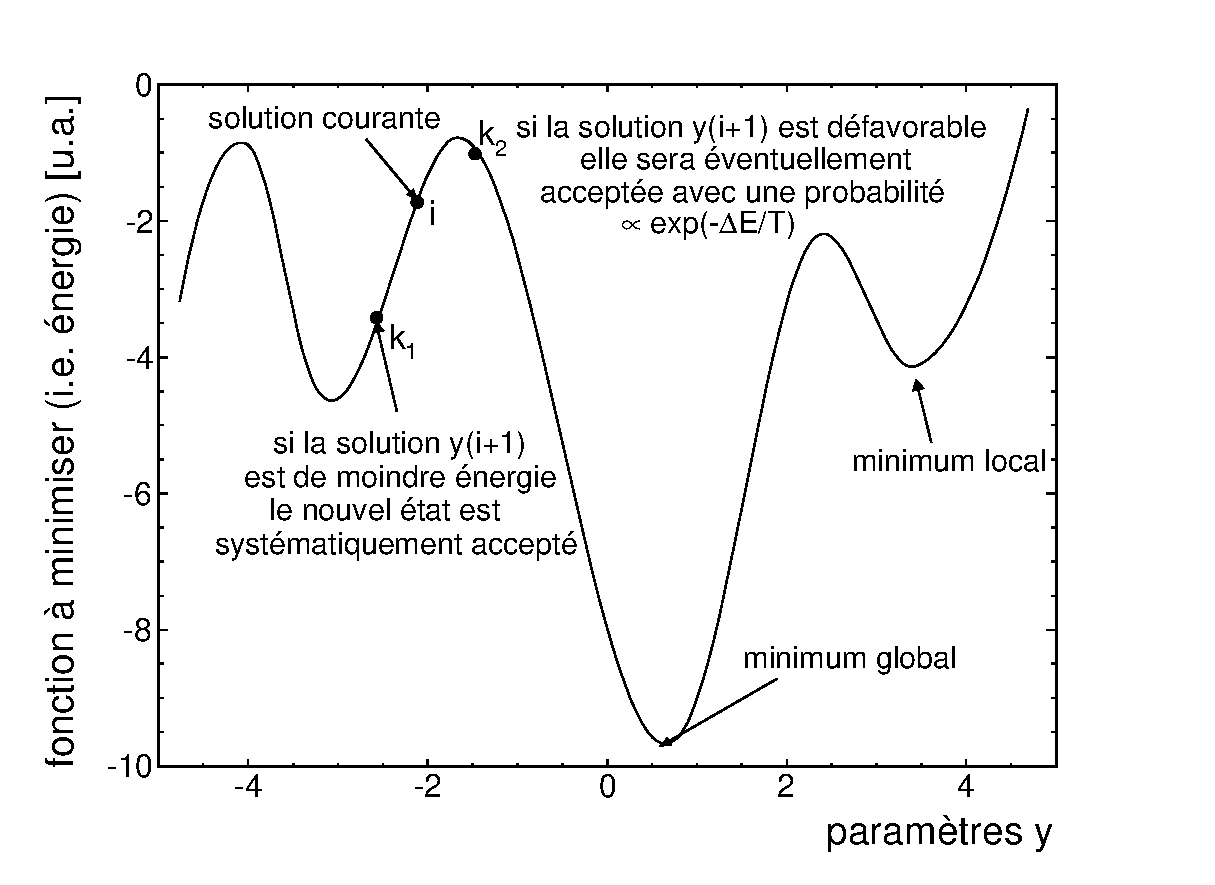
\includegraphics[scale=0.7]{./plot/PrincipleSAM}
  \caption{\textbf{Détermination d'un nouvel état pour la méthode de
      "recuit simulé".}}
  \label{fig:SAMPrinciple}
\end{figure}

\section{Forces et faiblesses de la méthode de "recuit simulé"}

En tant que technique générale d'optimisation, la méthode de "recuit
simulé" apporte une solution appropriée aux modèles hautement
non-linéaires, aux données bruitées ou soumises à de fortes
contraintes. L'un des ses principaux avantages vis-à-vis des méthodes
de régression tient à sa polyvalence étant donné que l'algorithme
Metropolis-Hastings sur lequel repose la méthode, ne s'appuie sur
aucunes propriétés intrinsèques au modèle. Ainsi, la méthode est tout
aussi efficace dans l'ajustement de fonctions
multi-paramètres~(\emph{cf.}~Partie~1 du projet) que dans
l'optimisation du parcours du voyageur de
commerce~(\emph{cf.}~Partie~2 du projet).

Cependant, il existe clairement un compromis entre "la qualité" de
la solution trouvée et le temps nécessaire à sa détermination. Si le
système est refroidit rapidement autrement dit si le temps de calcul
est court, l'algorithme peut se trouver alors "bloqué" dans un état
métastable relativement éloigné de l'état de moindre énergie. D'autre
part, plusieurs conditions sont requises afin de garantir la
convergence de la procédure. En particulier, les perturbations
aléatoires $\Delta\text{y}$ doivent être symétriques de façon à
assurer l'équivalence des chemins aller et retour \emph{i.e.}
\begin{equation*}
  p(\textbf{y}+\Delta\textbf{y}|\textbf{y})=p(\textbf{y}|\textbf{y}+\Delta\textbf{y})
\end{equation*}
Dans la pratique, on choisira donc des perturbations gaussiennes de
moyenne nulle et de variance fixe en prenant garde aux conditions aux
limites (par exemple, en faisant "rebondir" les paramètres aux
limites en utilisant la valeur absolue). Enfin, l'amplitude des
perturbations~$\Delta\textbf{y}$ relève d'un savant dosage afin que le
taux d'acceptation~(Ligne~5) ne soit ni trop grand de telle manière
que la chaîne stagne dans des minima locaux, ni trop faible
restreignant alors l'exploration de la distribution des
paramètres~$\textbf{y}$ à certaines valeurs. L'optimisation de la
convergence qui est en soi un domaine de recherches intensives revêt,
de ce point de vue, un intérêt et une attention
particulière\footnote{pour plus de détails, le lecteur intéressé
  pourra se référer aux ouvrages suivants~\cite{robert,marin,gilks}.}.

\section{Projet informatique associé à la méthode de "recuit simulé"}

\subsection{Préalable à l'utilisation de la méthode}

Dans un premier temps, le projet consistera en l'implémentation de la
méthode de "recuit simulé". Pour ce faire, on définira une classe
abstraite \lstinline$OptimizationMethod$ contenant les méthodes
virtuelles pures d'initialisation, d'exécution et de finalisation. On
définira ensuite une classe \lstinline$SimulatedAnnealing$, héritant
des propriétés de la classe \lstinline$OptimizationMethod$, et
spécifiant les métho\-des et les membres. On fera en sorte que les
paramètres inhérents à la méthode de "recuit simulé" (amplitude des
perturbations, températures initial et final, taux de refroidissement)
puissent être lus \emph{via} un fichier texte indépendant. D'autre
part, on définira une classe abstraite \lstinline$CostFunction$ dont
hériteront les fonctions à minimiser ($\chi^2$,...). Les définitions
des fonctions à minimiser seront donc données \emph{via} la
redéfinition des méthodes de \lstinline$CostFunction$. Le choix de la
fonction à minimiser devra également se faire à l'aide du fichier
texte de paramètres. Le modèle à optimiser appartiendra quant à lui à
une classe \lstinline$OptimizationModel$ comprenant les paramètres du
modèle (ex. les coefficients d'une droite) et les méthodes permettant
de les extraire. On oubliera pas de privilégier l'utilisation
d'énumérateurs afin de rendre la sélection des méthodes et des modèles
d'optimisations la plus transparente possible.

\subsection{Première partie du projet : ajustement de fonction multi-paramètres}

Il s'agit de tester l'efficacité de la méthode de "recuit simulé"
dans l'ajustement de données. Dans un premier temps, un programme
génère des données suivant une loi quelconque dont on cherche à
retrouver les paramètres \emph{via} la méthode de "recuit
simulé". Typiquement, un nombre $N$ de points sont tirés suivant une
loi linéaire, l'algorithme devant déterminer le coefficient directeur
de la droite et son ordonnée à l'origine. Par la suite, des jeux de
données issus de loi plus complexes pourront être simulés et
reconstruits. On évaluera et commentera notamment la variation du coût
en fonction du nombre d'itérations (comportement, convergence). On
pourra finalement ajouter aux jeux de données un bruit gaussien et
voir dans quelle mesure l'agorithme de "recuit simulé" reconstruit
les paramètres du modèle.

\subsection{Deuxième partie du projet : le problème du voyageur de commerce}

Dans la seconde partie du projet, la méthode de "recuit simulé" est
appliquée au problème du voyageur de commerce. L'exercice consiste,
étant donné un ensemble de villes séparées par des distances données,
à déterminer le plus court chemin reliant toutes ces villes. \'Enoncé
sous forme de jeu par William Rowan Hamilton en 1859, ce problème
d'optimisation combinatoire a historiquement été résolu grâce à la
méthode de "recuit simulé". On proposera différentes configurations où
le nombre de villes $N$ variera et on évaluera l'efficacité de
l'algorithme. Visuellement, on pourra sauvegarder les itérations
successives afin de représenter l'évolution du chemin parcouru par le
voyageur.

\def\etal{\textit{et al.}}

\renewcommand{\bibname}{References}

\begin{thebibliography}{9}
  \bibliographystyle{unsrt}

\bibitem{kirk1} S.~Kirkpatrick, C.~D.~Gelatt and M.~P.~Vecchi, {\em
  Optimization by Simulated Annealing}, Science, vol. 220, pp. 671-680 (1983)

\bibitem{kirk2} S.~Kirkpatrick, {\em Optimization by Simulated
  Annealing: Quantitative Studies}, Journal of Statistical Physics,
  vol. 34, pp. 975-986 (1984)

\bibitem{metro} N.~Metropolis \etal, {\em Equations of State
  Calculations by Fast Computing Machines}, Journal of Chemical
  Physics, vol. 21, pp. 1087-1092 (1953)

\bibitem{hastings} W.~K.~Hastings, {\em Monte Carlo sampling methods
  using Markov chains and their applications}, Biometrika, vol. 57,
  pp. 97-109 (1970)

\bibitem{robert} C.~P.~Robert and G.~Casella, {\em Monte Carlo
  Statistical Methods}, Springer-Verlag, 2004

\bibitem{marin} J.-M.~Marin and C.P.~Robert, {\em Bayesian Core: A
  Practical Approach to Computational Bayesian Statistics},
  Springer-Verlag, 2007

\bibitem{gilks} W.~R.~Gilks, S.~Richardson and D.~Spiegelhalter, {\em
  Markov Chain Monte Carlo in Practice}, Chapman \& Hall, 1996

\bibitem{rosenthal} J.~S.~Rosenthal, {\em Optimal Proposal
  Distributions and Adaptive MCMC}, Chapter for MCMC Handbook,
  S. Brooks, A. Gelman, G. Jones, and X.-L. Meng, eds.

\bibitem{roberts} G.~O.~Roberts and J.~S.~Rosenthal, {\em Examples of
  Adaptive MCMC}, to be print


\end{thebibliography}


\end{document}

% Local Variables:
% mode: latex
% coding: utf-8-unix
% End:
